\thispagestyle{plain}
\section{Metabolic Networks} \label{section:metabolic_networks}
\todo[inline]{brief introduction, shorten intro section, refer to book}
\unsure[inline]{index of v and G differ as they do not have the same length}
\todo[inline]{textsf for problems?}
% \begin{itemize}
%     \item chemical interactions between many of these components are now known and this knowledge gives rise to reconstructed biochemical reaction networks on a genome-scale that underlie various cellular functions
%     \item focus of systems biology on the nature of the links that connect them and on the functional states of the biochemical networks that result from the collection of all such links
%     \item Completing the relationship between all the chemical components of a cell, with their genetic bases, and its physiological functions is the promise of (molecular) systems biology
%     \item genotype: collection of all the genes and the particular
%     version of them found in a genome of an individual organism
%     \item phenotype: form and function of an organism
%     \item possible, in principle, to identify all the gene products
%     that make up an organism
%     \item reconstruct, on a genome-scale, metabolic networks for a
%     target organism in a biochemically detailed fashion ->  can be converted into a mathematical format yielding mechanistic genotype–phenotype relationships for microbial metabolism
%     \item BiGG models represent the reconciliation of the known biochemical properties of the gene products expressed in an organism
%     \item genome-scale models enable the computation of phenotypic traits based on the genetic composition of the target organism
%     \item Cellular functions rely on the coordinated action of the multiple gene products.
% \end{itemize}

% Understanding which chemical reactions take place in an organism, known as \textit{metabolism},  helps to understand cellular behaviour and cellular regulation. Metabolic analysis is important for drug discovery \todo[inline]{Mo: bioprocess optimization, strstrain design, etc.}, as the cellular function often is affected in a disease \cite{fba_applications_and_challenges}.

\textit{Computational systems biology} studies biological systems and biological networks by building and analysing mathematical models that approximate their behaviour \cite{intro_computational_systems_biology}. In this thesis we focus on models at the cellular level.
Instead of looking at the function of all molecules in a cell individually, as in molecular biology, systems biology studies the entire system and especially the links between the different cellular components \cite{palsson_systems_biology}. 
Looking at the system as a whole leads to a different understanding of the cell, as the behaviour of the cell depends on the interaction of the different components and cannot be explained by only studying the function of components individually \cite{intro_computational_systems_biology}.\\
In many cells, the chemical reactions that take place in an organism, known as \textit{metabolism}, determine the central function of the cell \cite{intro_computational_systems_biology}. Understanding the metabolism is therefore necessary in order to understand the cellular behaviour. 
% \todo[inline]{s the central function of a vast majority of cells; therefore, modelling metabolic networks can provide deep insights both into the behaviour of individual organisms \cite{intro_computational_systems_biology}}
% When studying a single cell, we are interested in the internal metabolite concentration, which depends on internal metabolites and reactions \todo[inline]{strange sentence}. 
\textit{Metabolites} are small molecules that are involved in metabolic reactions \cite{intro_computational_systems_biology}. We differentiate between \textit{internal reactions}, involving only internal metabolites, and \textit{exchange reactions}%\todo[inline]{Mo: explain why pseudo reactions}
. Exchange reactions are pseudo reactions representing the transport of metabolites, where either nutrition is taken up or a product is discarded by the cell \cite{fba_applications_and_challenges} \unsure[inline]{is this true in general or just for COBRA models?}. 
In a reaction, a set of metabolites called \textit{reactants} are converted into a different set of metabolites called \textit{products}. The \textit{stoichiometry} is the relative number of metabolites in a reaction. $Enzymes$ are important for the cell metabolism as they \textit{catalyze} reactions, which means that they accelerate reactions without being consumed by it.\\
Graphs can be used to model and understand cellular behaviour \cite{intro_computational_systems_biology}.
In a \textit{metabolic network}, the nodes are metabolites %, called \textit{metabolites}
and the edges represent reactions. 
A \acfi{gem} or \textit{enzyme constrained metabolic model} is a graph that contains all known metabolic information of a biological system such as reactions, metabolites and enzymes \cite{GEMs}.\\ 
The information required to build a GEM comes from a \textit{genome-scale reconstruction}, which is the process of identifying the genome of the organism including different components such as the stoichiometry, reaction direction and the corresponding catalyzing enzymes \cite{fba_applications_and_challenges} \unsure[inline]{about sentence}. 
Depending on the data and assumptions integrated in a model, a different accuracy is achieved, and different questions can be answered \cite{fba_applications_and_challenges}. 
% If one is interested in the dynamics of a system, for example how the metabolite concentration in a cell changes over time, a dynamic model is required. Dynamic models are usually based on differential equations and a large amount of model parameters is required to capture the complexity of a system \cite{intro_computational_systems_biology}.

In this thesis, we focus on constraint-based approaches, also known as \acfi{cobra}. A constraint excludes biologically unrealistic behavior, such as violating the laws of thermodynamics or the conservation of mass \cite{intro_computational_systems_biology}.
With constraint-based methods, one can predict the 
% or \textit{flux distribution} or \textit{reaction rate} %\unsure[inline]{correct?} 
rate of each reaction in the metabolic network \cite{intro_computational_systems_biology}.
% \todo[inline]{quick note on thermodynamics}
The mathematical representation of a metabolic network is described in \cref{section:mathematical_representation}.
The COBRA models relevant for this thesis are presented in \cref{section:optimization_gems}.

\subsection{Mathematical Representation} \label{section:mathematical_representation}
A \textit{hypergraph} $\mathscr{H}$ is defined by its set of vertices $\mathscr{V}$ and set of hyperedges $\mathscr{E}$. A hyperedge is a pair $E_i= (H_i,T_i)$ of disjoint subsets of $\mathscr{V}$, where $H_i$ denotes the vertices in the \textit{head} and $T_i$ the vertices in the \textit{tail}. A path is a sequence of vertices and hyperedges $P_{v_i,v_{q+1}} = (v_i, E_i, ..., E_{j-1}, v_j, E_{j}, ..., E_q, v_{q+1})$ where $v_i \in T_i$, $v_{q+1} \in H_q$ and $v_j \in T_j \cap H_{j-1}$ for all $j = 2,...,q$. A path is a cycle if $v_{q+1}$ is in the tail of $E_i$ \cite{gallo_directed_1993}.\\ %\unsure[inline]{add visualization?} 
A metabolic network $\mathcal{N}$ can be modeled as a hypergraph and is represented by the tuple ($\mathcal{M}, \mathcal{R}, \bold S, \bold l, \bold u$), where $\mathcal M$ is the set of internal metabolites and $\mathcal{R}$ is the set of reactions. The \textit{stoichiometric matrix} $\bold S \in \mathbb{R}^{m\times n}$ captures the entire network, where $m$ is the number of internal metabolites and $n$ is the number of reactions, including internal reactions $\mathcal{I}$ and exchange reactions $\mathcal{E}$. Usually, the number of metabolites is much smaller than the number of reactions \cite{intro_computational_systems_biology}. 
The columns of $\bold S$ correspond to the reactions in the network and the entries are the stoichiometric coefficients for each reaction and capture the mass balance for each metabolite. A negative coefficient indicates that a metabolite is consumed, called \textit{reactant} and is in the tail of the hyperedge. Vice versa, if the coefficient is positive, the metabolite is produced, called \textit{product}, and belongs to the head of the hyperedge.\\
\cref{fig:simple_model} shows a simplified metabolic network with three exchange reactions $\{r_1, r_4, r_8\}$ and five internal reactions $\{r_2, r_3, r_5, r_6, r_7\}$. The set of internal metabolites is $\{A, B, C, D, E, F\}$. The set of reversible reactions is $\{r_5, r_6, r_3\}$ and the set of irreversible reactions $\{r_1, r_2, r_4, r_7, r_8\}$. All irreversible reactions have to be greater or equal to zero. The metabolic network contains the cycle $(A, r_2, E, r_6, D, r_5, A)$.

\begin{figure}[h!]
    \centering
    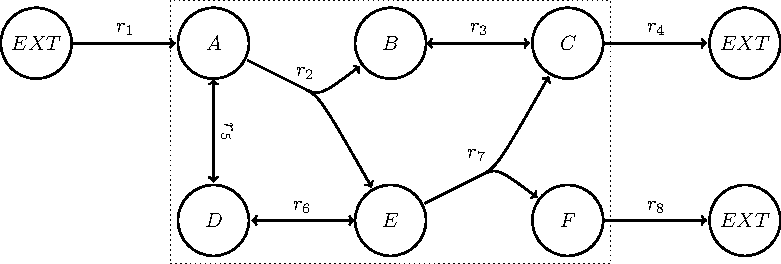
\includegraphics[width=0.8\textwidth]{Images/tikz_graphs_model_with_hyperarcs.pdf}
    \caption{Simplified metabolic network}
    \label{fig:simple_model}
\end{figure}

The corresponding stoichiometric matrix $\bold S$ is:
\begin{equation*}
    \bold S =
    \left[\begin{array}{cccccccc}
        1 & -1 & 0 & 0 & -1 & 0 & 0 & 0\\
        0 & 1 & -1 & 0 & 0 & 0 & 0 & 0\\
        0 & 0 & 1 & -1 & 0 & 0 & 1 & 0\\
        0 & 0 & 0 & 0 & 1 & -1 & 0 & 0\\
        0 & 1 & 0 & 0 & 0 & 1 & -1 & 0\\
        0 & 0 & 0 & 0 & 0 & 0 & 1 & -1\\    
    \end{array}\right]        
\end{equation*}

$\bold S$ is a $6 \times 8$ matrix, where the rows correspond to the internal metabolites in alphabetical order, and the columns denote the reactions $r_i$ in increasing order. In the exchange reaction $r_1$, $A$ is produced, and therefore the corresponding column has a positive entry for $A$. In the internal reaction $v_2$, the consumption of $A$ is captured by a $-1$ and the production of $B$ and $E$ are denoted by a 1 for each metabolite. In this example the quantities for the metabolites are either 0, 1 or -1 in all reactions. In more realistic metabolic models, the stoichiometric coefficients are still integer, but typically vary.
% \unsure[inline]{write bounds explicitly?}

The matrix $\bold S_\mathcal{I}$ is the submatrix of $\bold S$ that contains the columns of internal reactions only. 
The stoichiometric matrix $\bold S$ relates the flux\footnote{\textit{Flux}, \textit{reaction rate} and \textit{flux distribution} are used interchangeably throughout the thesis.} vector $\bold v$ to the change in metabolite concentration $\bold x$: $\frac{d \bold x}{dt} = \bold S \bold v$ \cite{noor_removing_2018}. The vector of flux distributions indicates the units of flow through all reactions. The vectors $\bold l$ and $\bold u$ capture the lower and upper bounds of the flux for all reactions. If the direction of a reaction is forced in one direction by the bounds, the reaction is said to be \textit{irreversible}. Otherwise, it is \textit{reversible}.
The metabolic fluxes are given in units of $\frac{\text{mmol}}{\text{gDW} \times \text{h}}$, which denotes the flux of a metabolite normalized to the biomass of the cell.
%amount of metabolites per hour. 
%which is the concentration per gram dry weight and hourich is the concentration per gram dry weight and hour

\subsection{Optimization for Metabolic Networks} \label{section:optimization_gems}
% \todo[inline]{start with PDE (metabolites are variables) and cobra (fluxes are variables)}
% \todo[inline]{define flux with v = ... ODE paramaters => parameters drop in optimization approach}
% Once a mathematical representation of a model is available, one question is which reaction rates are possible and likely to occur in an organism. 
In dynamic modelling, the dynamics of metabolite concentration are expressed by kinetic laws and kinetic parameters \cite{intro_computational_systems_biology}: 
\begin{equation} \label{Eq:dynamic_model}
    \frac{dx_i}{dt} = f_i(x_1, x_2, ..., x_n; \Theta)
\end{equation}
\quad where $\Theta$ is the set of kinetic parameters and $f_i$ models how the concentration of $x_i$ changes depending on the concentration of the other metabolites. Such a dynamic model requires a lot of computational data in order to predict the metabolite concentration $\bold x$.
% \todo[inline]{dynamic modelling: observe dynamics of a system in terms of the changes in levels of metabolites/genes/proteins \\ require species and interactions -> for each interaction in the model, the right kind of kinetics must be chosen \cite{intro_computational_systems_biology}}

In constraint-based reconstruction and analysis (COBRA) methods, dynamic metabolic networks are modeled at \textit{steady-state}: 
\begin{equation*}
    \frac{d \bold x}{dt} = \bold S \bold v= \bold 0 
\end{equation*} 
\quad where $\bold v \in \mathbb{R}^n$ is the vector of flux distributions, and the stoichiometric matrix $\bold S \in \mathbb{R}^{m \times n}$ captures the topology of the metabolic network. In COBRA methods, the set of possible flux distributions is analysed mathematically, whereas in dynamic modelling, the metabolite concentration is predicted. With COBRA methods one can predict the flux distribution under different environmental conditions and under changes in the environment \cite{intro_computational_systems_biology}.
% \todo[inline]{Constraint-based modelling is focussed on metabolic networks and is most useful to predict the growth rate of a cell, under specific environmental conditions, such as given glucose uptake rate, or following perturbations, such as the knock-out of certain genes from an organism.}
% \todo[inline]{m < r in real metabolic networks. This is because the same metabolites mix and match in different reactions; further, many sink reactions that represent the exchange of intracellular metabolites are always present in the model. Thus, we commonly are confronted with a situation where the number of unknowns is much higher than the number of equations, i.e. the system of linear equations is under-determined. \cite{intro_computational_systems_biology}}
\\
Apart from the steady-state assumption, COBRA methods use context-specific constraints such as \textit{reaction flux bounds} and \textit{mass conservation}. % and the \textit{steady-state assumption} \cite{cobrapy}. 
Mass balance is captured in the stoichiometric matrix $\bold S$. 
%a balance of the produced and consumed metabolite concentration. 
As metabolic reactions take place fast compared to other reactions, such as cell division, the steady-state assumption is biologically plausible \cite{enumerate_extreme_rays}. Compared to the dynamic modeling in \cref{Eq:dynamic_model}, COBRA methods require much less experimental data \cite{intro_computational_systems_biology}.\todo[inline]{reduntant with info in previous paragraph} \todo[inline]{check with optimization section, mention dimension}

% As the number of metabolites $m$ is smaller than the number of reactions $n$, the resulting system of linear equations is underdetermined \cite{intro_computational_systems_biology} 
\textit{Extreme pathways} are a set of vectors that satisfy the model constraints, such that any feasible flux can be written as a convex combination of extreme pathways \cite{price_extreme_2002}.
% The steady-state assumption defines a polyhedral feasible region. The extreme points of the polyhedron are called \textit{extreme pathways}.
There are three types of extreme pathways: \textit{primary systemic pathways} (Type \rom{1}), \textit{futile cycles} (Type \rom{2}) and \textit{internal cycles} (Type \rom{3}). \cref{fig:extreme_pathways} shows the difference between the extreme pathways.
Primary systemic pathways are pathways where exchange reactions are used%\unsure[inline]{should it be two?}
\cite{noor_removing_2018}. These pathways are thermodynamically feasible and are desirable steady-state flux solutions (see \cref{section:ll_fba}). 
For most COBRA methods, the goal is to compute a Type \rom{1} pathway and forbidding Type \rom{2} and Type \rom{3} pathways.\\
In order to understand the difference between Type \rom{2} and Type \rom{3} pathways, we have to introduce \textit{currency exchange reactions}. Currency exchange reactions are a subset of internal reactions, where the currency within the cell is changed \cite{noor_removing_2018}. For example, a reaction, where ATP is generated from ADP, transfers energy and is a Type \rom{2} pathway.\\
Internal cycles are pathways where none of the exchange reactions and none of the currency exchange reactions are used and are thermodynamically infeasible. 
%and are not wanted as steady-state flux solutions
%between different sub-networks in the cell is exchanged. 
Futile cycles are pathways where none of the exchange reactions is used, but at least one currency exchange reaction is used \cite{noor_removing_2018}. \textit{Energy reducing cycles} are futile cycles that are biologically feasible and should be allowed solutions, whereas \textit{energy generating cycles} (EGCs) are futile cycles that are not wanted in a solution \cite{noor_removing_2018}. EGCs are problematic as they can lead to solutions that have a better objective value than when restricting the use of EGCs. One possibility to prevent EGCs is to force the directionality of the reaction. 

\begin{figure}[h!]
    \centering
    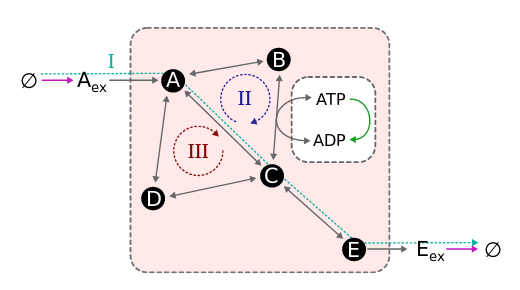
\includegraphics[width=0.6\textwidth]{Images/extreme_pathways.png}
    \caption{Types of extreme pathways}
    \label{fig:extreme_pathways}
    \subcaption*{The figure is taken from \cite{noor_removing_2018}.Primary systemic pathways (Type \rom{1}) are biologically realistic, whereas internal cycles (Type \rom{3}) are not thermodynamically feasible. Futile cycles (Type \rom{2}) can either generate energy or reduce energy. Energy generating cycles are thermodynamically infeasible, whereas energy consuming cycles are realistic.}
\end{figure}
% \unsure[inline]{Mo: all internal cycles are bad}

The feasible region of a COBRA model usually contains multiple solutions. We are interested in flux distributions that optimize a biological objective. A commonly used objective function is the maximization of growth. Growth can be incorporated into the stoichiometric matrix $\bold S$ by adding an extra column where the coefficients indicate the contribution to growth \cite{FBA}. For an overview of biological objectives, see \cite{palsson_systems_biology}.

Depending on the constraints and the objective, we obtain a different COBRA variant. Each corresponds to an optimization problem which can be solved with methods described in \cref{section:optimization}. Several COBRA methods relevant for this thesis are explained below.

\subsubsection{Flux Balance Analysis} \label{section:fba}
The most basic COBRA method is \acfi{fba}. An optimal solution $\bold v^*$ to an \textsf{FBA} model, is a flux distribution maximizing a biological linear objective which respects the steady-state assumption and bound constraints.

\begin{maxi!}
  {\scriptstyle \bold v}{\bold c^\intercal \bold v}{\text{\textbf{FBA}} \label[problem]{problem:fba}}{}
    \addConstraint{\bold S \bold v= \bold 0} \label[constraint]{constraint:fba_b}
    \addConstraint{\bold l \leq \bold v \leq \bold u}
\end{maxi!}
\myproblems{\textsf{FBA} - \cref{problem:fba}}

where $\bold c \in \mathbb{R}^n$ determines the linear objective function of the FBA. The structure of the network is captured in the stoichiometric matrix $\bold S$. The fluxes $\bold v \in \mathbb{R}^n$ are bounded by $\bold l, \bold u \in \mathbb{R}^n$. \cref{constraint:fba_b} ensures the steady-state of the metabolite concentration. We are dealing with a linear program which can be solved efficiently (see \cref{section:Linear Programming}).

As an example, let us consider the metabolic network in \cref{fig:loop}. We have three internal metabolites $A,B,C$, two irreversible exchange reactions $r_1, r_5$ and three reversible internal reactions $r_2, r_3, r_4$. The stoichiometric matrix is: 

\begin{equation} \label{Eq:S_loop}
    \bold S =
    \left[\begin{array}{ccccc}
        1 & -1 & 0 & -1 & 0 \\
        0 & 1 & -1 & 0 & 0 \\
        0 & 0 & 1 & 1 & -1 \\
    \end{array}\right]        
\end{equation}

\quad and we assume the following bounds on the fluxes: 
\begin{equation} \label{Eq:bounds_loop}
    \bold l = (0,-30,-30,-30,0) \quad \bold u = (10,30,30,30,10)
\end{equation}

\begin{figure}[h!]
    \centering
    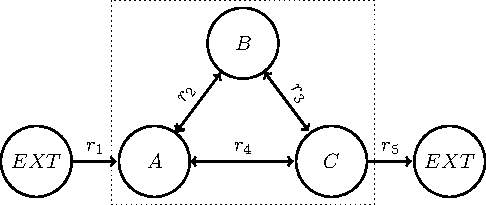
\includegraphics[width=0.6\textwidth]{Images/tikz_graphs_one_loop.pdf}
    \caption{Simple model with internal loop}
    \label{fig:loop}
\end{figure}

If we maximize the flux through the internal reactions, that is $\bold c = (0,1,1,1,0)$, an optimal solution is $\bold v^* = (10, 30, 30, -20, 10)$. The solution contains an internal loop, as there is a flux of 20 going through each of the internal reactions, as seen in \cref{fig:loop_solutions}.

\begin{figure}[H]
    \centering
    \label{fig:loop_solutions}
    \begin{subfigure}{0.5\textwidth}
    \centering
        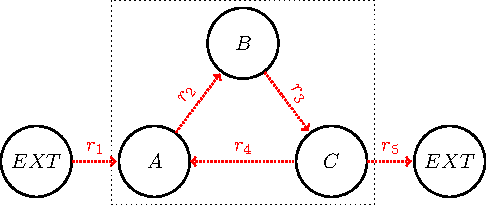
\includegraphics[width=0.99\linewidth]{Images/tikz_graphs_one_loop_fba.pdf}
        \caption{}
    \end{subfigure}%
    \begin{subfigure}{0.5\textwidth}
    \centering
        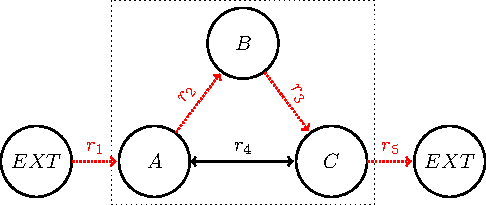
\includegraphics[width=0.99\linewidth]{Images/tikz_graphs_one_loop_ll_fba.pdf}
        \caption{}
    \end{subfigure}
    \caption{Used reactions in the \textsf{FBA} solution (a) which contains an internal cycle, and used reactions in the \textsf{ll-FBA} solution (b).}
\end{figure}

A solution to \textsf{FBA} can be a convex combination of primary systematic pathways, futile cycles and internal cycles. To prevent biologically implausible futile cycles, the directionality is restricted with the bound constraints \cref{problem:fba} (c). Internal cycles are biologically not realistic, but are part of the solution space, posing a major drawback to \textsf{FBA} solutions. 

% \subsubsection{Parsimonous FBA}
% \todo[inline]{add mathematical model}
% \todo[inline]{link to CycleFreeFlux}

\subsubsection{CycleFreeFlux} \label{section:molecular_networks_cyclefreeflux}
Suppose we are given a solution $\bold v^{FBA}$ to an \textsf{FBA} problem (\cref{problem:fba}). 
The following linear program, known as \acfi{cff}, returns a solution $\bold v$ that is structurally consistent with $\bold v^{FBA}$ and with the minimum sum of reaction rates such that the objective values are identical \cite{desouki_cyclefreeflux_2015-1}. 

\begin{mini!}
    {\scriptstyle \bold v}{\sum_i |v_i| = \sum_{i: v_i^{FBA} > 0} v_i - \sum_{i: v_i^{FBA} < 0} v_i}{\text{\textbf{CFF}} \label[problem]{problem:CycleFreeFlux}}{} 
    \addConstraint{\bold S\bold v= \bold 0} \label[constraint]{constraint:CFF_1}
    \addConstraint{{\bold c^\intercal \bold v} = {\bold c^\intercal \bold v}^{FBA}} \label[constraint]{constraint:CFF_2}
    \addConstraint{0 \leq v_i \leq v_i^{FBA} \quad \text{for $i$ with $v_i^{FBA} \geq 0$}} \label[constraint]{constraint:CFF_3}
    \addConstraint{v_i^{FBA} \leq v_i \leq 0 \quad \text{for $i$ with $v_i^{FBA} < 0$}} \label[constraint]{constraint:CFF_4}
    \addConstraint{v_i = v_i^{FBA} \quad \forall i \in \mathcal{E}} \label[constraint]{constraint:CFF_5}
\end{mini!}
\myproblems{\textsf{CFF} - \cref{problem:CycleFreeFlux}}
Beside the steady-state assumption in \cref{constraint:CFF_1}, the reaction direction has to match the direction in $\bold v^{FBA}$ or become zero, enforced by \cref{constraint:CFF_3} and \cref{constraint:CFF_2}. In addition, the reaction rates of the exchange reactions $\mathcal{E}$ remain unchanged (\cref{constraint:CFF_5}).
\cref{constraint:CFF_2} ensures that the objective value of $\bold v$ matches the objective value of $\bold v^{FBA}$. The objective function can be rewritten by replacing the absolute function by the sum of positive reaction rates minus the sum of negative reaction rates, as the sign of reaction rates is known from $\bold v^{FBA}$. As \cref{problem:CycleFreeFlux} is a linear program, it is easy to solve (see \cref{section:solving_lps}). 
If the reactions contained in an internal loop are allowed to be zero, and  if the objective does not depend on a reaction which is contained in an internal loop%, and if the model does not contain energy-generating cycles
, $\bold v$ is thermodynamically feasible \cite{noor_removing_2018}. \unsure[inline]{other cases or disadvantages?}

Let us go back to the \textsf{FBA} example visualized in \cref{fig:loop}. If we apply \textsf{CycleFreeFlux} to the \textsf{FBA} solution $\bold v^{FBA} = (10,30,30,-20,10)$ with $\bold c^\intercal \bold v^{FBA} = 40$, the solution flux 
$\bold v^* = (10,30,30,-20,10)$ still contains an internal loop.

We will see in \cref{section:ll_fba} that formulating a mathematical program such that the resulting flux is in the thermodynamically feasible subspace is $\mathcal{NP}$-hard.

As explained in \cite{desouki_cyclefreeflux_2015-1}, the \textsf{CycleFreeFlux} algorithm can be used to enumerate cycles. For each internal reaction $i$, we solve three LPs. 
We first solve an \textsf{FBA} problem, where we maximize the flux through reaction $i$, whose solution is denoted by $\bold v^{FBA}$. We solve the \textsf{CFF} problem based on $\bold v^{FBA}$, whose solution is denoted by $\bold v^{CFF}$. If $\bold v^{FBA} \neq \bold v^{CFF}$, we know that $\bold v^{FBA}$ contains an internal cycle. We solve another \textsf{CFF} problem based on $\bold v^{FBA}$ with the additional constraint $v_i = v_i^{FBA}$, whose solution is denoted by $\bold v^{(2)}$. The solution $\bold v^{CFF}$ contains one internal cycle, which corresponds to the difference between $\bold v^{(2)} - \bold v^{CFF}$.
\todo[inline]{rename v(2)?}

% \unsure[inline]{how to present paper? Mention complexity of ll-FBA}
% \todo[inline]{mention FVA; FVA possible with cyclefreeflux; mention parsimonous FBA}
% \todo[inline]{compare to parsimonous fba}



% Assuming that no reaction in a loop is maximized in the objective and such reactions are allowed to carry zero flux, 
% solving the LP for a given FBA solution, provides a test for thermodynamic feasibility: $\bold v^{FBA}$ is thermodynamically feasible if $\bold v= \bold v^{FBA}$, where $v$ is the solution to \eqref{problem:CycleFreeFlux}.
% And in that case \eqref{problem:CycleFreeFlux} can be used to enumerate thermodynamically infeasible cycles.  

\subsubsection{Thermodynamic Flux Balance Analysis}
The second law of thermodynamics states that the entropy in a closed system cannot decrease. In a metabolic network, each reaction $i$ is associated with a scalar $\Delta \mu_i$ denoting the \textit{Gibbs free energy change} %\todo[inline]{use Gibbs free energy change everywhere} 
or \textit{potential difference}.
The following has to hold \cite{elimination_infeasible_loops}: 
\begin{equation*}
    \Delta \mu_i = \Delta \mu \degree_i + RT \mathrm{ln} (Q_i)
\end{equation*}

$R$ is the universal gas constant, which relates energy to the amount of substance and temperature, and $T$ the temperature in Kelvin. $Q_i$ is the reaction quotient and denotes the ratio of product concentration to reactant concentration. $\Delta \mu \degree_i$ is the \textit{standard chemical potential}, or \textit{equilibrium potential}, or \textit{standard Gibbs free energy} of reaction $i$.
Instead of using the reaction quotient, we can calculate the concentration of reactants and products in reaction $i$ by using the stoichiometric coefficients $s_{i,*}$ and the metabolite concentration $\bold c$ \cite{noor_removing_2018}:
\begin{equation*}
    \Delta \mu_i = \Delta \mu \degree_i + RT \sum_{i} s_{i,*}^\intercal \mathrm{ln} (\bold c)
    \label{Eq:lawOfThermodynamics}
\end{equation*}
where $\Delta \mu_i$ is the change of Gibbs free energy for reaction $i$. \\
Written in matrix notation, we have:
\begin{equation}
   \boldsymbol{\Delta \mu} = \boldsymbol{\Delta \mu \degree} + RT \bold S^\intercal \mathrm{ln}(\bold c)
\end{equation}

One method that integrates thermodynamic data to get solutions that are thermodynamically feasible is \textit{thermodynamic flux balance analysis} (TFBA). 

\begin{maxi!}
  {\scriptstyle \bold v, \bold a, \bold x, \boldsymbol \mu}{\bold c^\intercal \bold v}{\text{\textbf{TFBA}} \label[problem]{problem:tfba}}{}
    \addConstraint{\bold S \bold v= \bold 0} \label[constraint]{constraint:tfba_1}
    \addConstraint{\bold l \leq \bold v \leq \bold u} \label[constraint]{constraint:tfba_2}
    \addConstraint{0 \leq M \bold a_i-\bold v_i \leq M \quad \forall i \in \mathcal{I}} \label[constraint]{constraint:tfba_3}
    \addConstraint{\epsilon \leq M \bold a_i + \boldsymbol{\Delta \mu_i} \leq M - \epsilon \quad \forall i \in \mathcal{I}} \label[constraint]{constraint:tfba_4}
    \addConstraint{\boldsymbol{\Delta \mu} = \boldsymbol{\Delta \mu \degree} + RT \bold S_{\mathcal{I}}^\intercal \bold x} \label[constraint]{constraint:tfba_5}
    \addConstraint{\mathrm{ln}(\bold b^L) \leq \bold c \leq \mathrm{ln}(\bold b^U)} \label[constraint]{constraint:tfba_6}
    \addConstraint{a_i \in \{0,1\}} \label[constraint]{constraint:tfba_7}
\end{maxi!}
The steady-state constraint (\cref{constraint:tfba_1}), the bound constraints (\cref{constraint:tfba_2}) and the linear objective function correspond to the \textsf{FBA} model (\cref{problem:fba}). \cref{constraint:tfba_3} and \cref{constraint:tfba_4} ensure that the Gibbs free energy is never reduced for any reaction $i$: $v_i = 0 \lor \text{sign}(v_i) = - \text{sign}(\Delta \mu_i)$. $M \in \mathbb{R}$ is a large constant that does not restrict the value of $\bold v$ and $\boldsymbol{\Delta \mu}$. The binary variables $\bold a$ indicate the direction of $\bold v$: $a_i=1$ implies $v_i>0$ and $a_i=0$ implies $v_i<0$. If $a_i=1$, $v_i$ is zero or positive as $-M \leq -v_i \leq M$ holds. $\Delta \mu_i$ is not allowed to be zero so it is bounded by a small value $\epsilon$. In that case, $\Delta \mu_i$ is negative as $\epsilon - M \leq \Delta \mu_i \leq - \epsilon$. If $a_i=0$, $0 \leq -v_i \leq M$ holds and the flux $v_i$ is zero or negative. $\Delta \mu_i$ is positive as $\epsilon \leq \Delta \mu_i \leq M - \epsilon$.
$\bold c$ is the vector of metabolite concentrations which is bounded by $\mathrm{ln}(\bold b^L)$ and $\mathrm{ln}(\bold b^U)$. 
\cite{noor_removing_2018}

A solution to a TFBA model is thermodynamically feasible, however the model requires the standard equilibrium potential for each reaction $\boldsymbol{\Delta \mu \degree}$ which is oftentimes not known. Additionally, the resulting problem is a mixed-integer problem and more difficult to solve than the \textsf{FBA} problem.

\newpage
\subsubsection{Loopless FBA} \label{section:ll_fba}
A simpler method to ensure that a solution does not contain an internal loop, which does not require additional thermodynamic data is \acfi{ll-fba}. 
To respect the second law of thermodynamics, the following inequality for reaction $i$ is required: 
\begin{equation}
    \{v_i = 0\} \lor \{\text{sign}(v_i) = - \text{sign}(\Delta \mu_i)\} 
\end{equation}
\quad which means that if a reaction carries flux, Gibbs free energy decreases \cite{muller_fast_2013}. 
A \textit{loop} is a nonzero flux vector $\boldsymbol \ell$ such that the internal network is at steady-state: $\bold S_{\mathcal{I}} \boldsymbol \ell = \bold 0$ \cite{noor_proof_2012}. As $\ell_i$ and $\Delta \mu_i$ have to be of opposite sign, unless $\ell_i=0$, we know that $\boldsymbol \ell^\intercal \boldsymbol{\Delta \mu} \neq \bold 0$. % sum of negatives and zeros will be negative
However, \textit{flux balance}, or \textit{Kirchhoff's second law}, states that the reaction energies around a circuit have to sum up to zero, and therefore $\boldsymbol \ell$ is not thermodynamically feasible \cite{elimination_infeasible_loops}. 
A flux distribution $\bold v$ contains a loop if there exists a nonzero vector $\boldsymbol \ell$ with $\bold S_{\mathcal{I}} \boldsymbol \ell = \bold 0$ such that: %$\ell_i=0$ or $\ell_i$ and $v_i$ have the same
\begin{equation*}
    \text{sign}(\ell_i) \in \{\text{sign}(v_i),0\} \quad \forall i \in \mathcal{I}
\end{equation*}

For a solution to be thermodynamically feasible, the reaction energies around any flux $\bold v$ have to sum up to zero: $\bold v^\intercal \boldsymbol{\Delta \mu} = 0$, where $\boldsymbol{\Delta \mu}$ is the vector of Gibbs free energy \cite{elimination_infeasible_loops}. As we are interested in internal cycles, it is sufficient to verify that $\bold v_\mathcal{I}^\intercal \boldsymbol{\Delta \mu} =0$, where $\bold v_\mathcal{I}$ is a flux distribution through internal reactions and $\boldsymbol{\Delta \mu}$ are the corresponding changes in Gibbs free energy.
Any steady-state nonzero pathway that just uses internal reactions is a loop: $\bold S_{\mathcal{I}} \bold v_{\mathcal{I}} = \bold 0$ \cite{noor_proof_2012}. The nullspace of $\bold S_{\mathcal{I}}$ is defined as $\mathrm{null}(\bold S_{\mathcal{I}}) := \{\bold x \in \mathbb{R}^{|\mathcal{I}|} : \bold S_{\mathcal{I}} \bold x = \bold 0 \}$. Let $\bold B \in \mathbb{R}^{|\mathcal{I}| \times n}$ be a matrix with columns formed by the set of vectors $\{\bold b_i\}_{i=1}^n$ that form a basis for $\mathrm{null}(\bold S_{\mathcal{I}})$. \todo[inline]{verify dimension}
Any loop $\boldsymbol \ell$ lies in the nullspace of $\bold S_{\mathcal{I}}$ and can thus be written as $\boldsymbol \ell = \bold B ^\intercal \boldsymbol \alpha$ \todo[inline]{transpse needed??}, where coefficients $\alpha_i \in \mathbb{R}$ \cite{elimination_infeasible_loops}. Therefore, the following removes solutions with internal loops: $\bold B^\intercal \boldsymbol{\Delta \mu} = \bold 0$. Adding the loopless constraints to the \textsf{FBA} problem, we obtain the following mathematical program:
\begin{maxi!}
    {\scriptstyle \bold v, \boldsymbol{\Delta \mu}}{\bold c^\intercal \bold v}{\label[problem]{problem:llfba_nullspace}}{}
    \addConstraint{\bold S \bold v= \bold 0} 
    \addConstraint{\bold l \leq \bold v \leq \bold u}
    \addConstraint{\Delta \mu_i v_i < 0 \lor v_i = 0  \quad \forall i \in \mathcal{I}}        
    \addConstraint{\bold B^\intercal \boldsymbol{\Delta \mu} = \bold 0} \label[constraint]{constraint:llfba_nullspace_e}
\end{maxi!}
\enlargethispage{1cm}
\quad where $\bold v \in \mathbb{R}^n$ and $\boldsymbol{\Delta \mu} \in \mathbb{R}^{|\mathcal{I}|}$. For readability, index $i$ corresponds to the pair of $v_i$ and $\Delta \mu_i$, even though $\bold v$ and $\boldsymbol{\Delta \mu}$ are of different length.
\todo[inline]{mention that v and delta mu are of different length, but i is specific index}

We can write \cref{constraint:llfba_nullspace_e} as $\boldsymbol{\Delta \mu} = \bold S ^\intercal \boldsymbol \mu$ \cite{noor_proof_2012, elimination_infeasible_loops, muller_fast_2013}. Let us define the vector of potential differences of the internal reactions as $\boldsymbol{\Delta \mu} = \bold S ^\intercal \boldsymbol \mu$, where $\boldsymbol \mu$ is approximately the chemical potential. Looking only at internal reactions, $\boldsymbol{\Delta \mu}$ is defined as $\boldsymbol{\Delta \mu} = \bold S_\mathcal{I}^\intercal \boldsymbol \mu$.  
Each vector in the rowspace of $\bold S_{\mathcal{I}}$ is orthogonal to each vector in the nullspace of $\mathrm{null}(\bold S_{\mathcal{I}})$ \cite{noor_proof_2012}.
Therefore, $\bold B^\intercal \boldsymbol{\Delta \mu} = \bold 0$. 
\todo[inline]{read paper again}

Rewriting \cref{constraint:llfba_nullspace_e}, we obtain the following mathematical program \cite{muller_fast_2013}:
\begin{maxi!}
    {\scriptstyle \bold v, \boldsymbol{\Delta \mu}, \boldsymbol \mu}{\bold c^\intercal \bold v}{\label[problem]{problem:llfba_original}}{}
    \addConstraint{\bold S \bold v= \bold 0} 
    \addConstraint{\bold l \leq \bold v \leq \bold u}
    \addConstraint{\Delta \mu_i v_i < 0 \lor v_i = 0  \quad \forall i \in \mathcal{I}}        
    \addConstraint{\boldsymbol{\Delta \mu} = \bold S_{\mathcal{I}}^\intercal \boldsymbol \mu} \label[constraint]{constraint:llfba_original_e}
    % \addConstraint{\mu \in \mathbb{R}^m}
    % \addConstraint{\Delta \mu \in \mathbb{R}^n}
    % \addConstraint{v \in \mathbb{R}^n}
    % \addConstraint{\bold S \in \mathbb{R}^{m\times n}}
\end{maxi!}
where $\boldsymbol \mu \in \mathbb{R}^m$ and $\boldsymbol{\Delta \mu} \in \mathbb{R}^{|\mathcal{I}|}$. 
\cref{problem:llfba_original} is $\mathcal{NP}$-hard and much more complicated to solve than \textsf{FBA} \cite{cornelis_metabolic_nodate}. We use $\boldsymbol{\Delta \mu}$ and $\boldsymbol \mu$ due to the biological interpretability, however it is not necessary to define $\boldsymbol{\Delta \mu}$ as it only appears in \cref{constraint:llfba_original_e}.

Constraint (d) in \cref{problem:llfba_original} and \cref{problem:llfba_nullspace} poses a challenge due to the disjunction, the strict equality and the product of decision variables $\boldsymbol{\Delta \mu}$ and $\bold v$. To simplify the model, the disjunction is rewritten and we arrive at the loopless FBA model used in this thesis.

\begin{maxi!}
    {\scriptstyle \bold v, \boldsymbol{\Delta \mu}, \boldsymbol \mu}{\bold c^\intercal \bold v}{\text{\textbf{ll-FBA}} \label[problem]{problem:llfba}}{}
    \addConstraint{\bold S \bold v= \bold 0} \label[constraint]{constraint:llfba_b}
    \addConstraint{\bold l \leq \bold v \leq \bold u} \label[constraint]{constraint:llfba_c}
    \addConstraint{\begin{aligned} &\bigl((v_i \geq 0) \land (\Delta \mu_i \leq - \epsilon) \bigr) \, \, \lor \\ 
    &\bigl((v_i \leq 0) \land (\Delta \mu_i \geq \epsilon) \bigr) \end{aligned} \quad \quad \forall i \in \mathcal{I}} \label[constraint]{constraint:llfba_d}
    \addConstraint{\boldsymbol{\Delta \mu}^\intercal = \boldsymbol \mu^\intercal \bold S_{\mathcal{I}}} \label[constraint]{constraint:llfba_e}
    % \addConstraint{\mu \in \mathbb{R}^m}
    % \addConstraint{\Delta \mu \in \mathbb{R}^n}
    % \addConstraint{v \in \mathbb{R}^n}
    % \addConstraint{\bold S \in \mathbb{R}^{m\times n}}
\end{maxi!}
\myproblems{\textsf{ll-FBA} - \cref{problem:llfba}}
Whereas the value of $\boldsymbol{\Delta \mu}$ in TFBA corresponds to the Gibbs free energy change tested in experiments, in ll-FBA only the $\text{sign}(\boldsymbol{\Delta \mu})$ corresponds to the actual Gibbs free energy change \cite{elimination_infeasible_loops}. 
As the value does not matter, we can scale $\boldsymbol{\Delta \mu}$ by not allowing it to be in the interval $[- \epsilon , \epsilon ]$.
The resulting problem is a disjunctive program with linear constraints in the disjunctions and can be reformulated as a mixed-integer program with indicator or big-M constraints (see \cref{section:solving_dps}). 

% \todo[inline]{explain why this is ok (M.)}
% \todo[inline]{cite proofs, especially complexity proof}

Going back to the previous example with $\bold S$ defined in \cref{Eq:S_loop} and flux bounds defined in \cref{Eq:bounds_loop},  
the loopless flux distribution is $\bold v^* = (10,10,10,0,10)$ with $\bold c^\intercal \bold v^* = 20$ which is shown in \cref{fig:loop_solutions}. 
\todo[inline]{fix reference}

Loopless FBA excludes internal cycles from the solution space. However, energy generating cycles still have to be blocked by restricting the directionality.

\subsubsection{st-FBA}
\textit{Semi-thermodynamic Flux Balance Analysis} (st-FBA) combines the loopless FBA and TFBA approaches \cite{noor_removing_2018}. The loopless FBA formulation is extended by constraining the Gibbs free energy change $\boldsymbol{\Delta \mu}$ of a subset of reactions. Metabolites that carry energy such as ATP and their related compounds such as ADP and AMP are treated as in TFBA. The chemical potential of such a metabolite is limited by bounds known from experiments. Bounding the chemical potential of these energy-carrying currency metabolites excludes energy generating cycles, and it is no longer required to force the direction of certain reactions as in ll-FBA. 
st-FBA is thus a trade off between the $\boldsymbol{\Delta \mu}$ values corresponding to the Gibbs free energy changes which requires experimental data, and the approximation of the Gibbs Free energy changes which only deals with the directionality.
We require more experimental data than for ll-FBA, as we need the bounds of reactions involved in energy reducing cycles. As we add the experimental data just on a small subset of reactions, just a fraction of information needed for TFBA is needed for st-FBA.
% \unsure[inline]{why S not in constraints (30)-(31)?}
% \todo[inline]{why model exists, advantages, disadvantages, compare to ll-FBA and TFBA (M.)}

\subsubsection{Enzyme Constrained Metabolic Models}
In FBA, the optimal reaction rate of a metabolic network is limited by the nutrition uptake. However, the flux depends also on the enzyme abundances catalysing the reactions. Especially modelling physiological responses, such as \textit{overflow metabolism}, requires enzymatic data \cite{improving_phenotype_predictions}. Overflow metabolism refers to the phenomenon that a cell uses fermentation instead of respiration, even though respiration is more energetically efficient \cite{overflow}. There are several hypotheses to explain the metabolic switch from respiration to fermentation. One hypothesis is that overflow metabolism is connected to the enzyme mass. When using fermentation, the cell does not grow as fast as with respiration, but it yields more energy with the same enzyme mass \cite{improving_phenotype_predictions}.  
\textit{GECKO} is one method that integrates enzyme constraints into a genome-scale model. The following section is based on \cite{improving_phenotype_predictions}. 

\newpage
Suppose reaction $j$ is catalysed by enzyme $E_i$. The \textit{turnover number} indicates how efficient an enzyme is. The reaction rate $v_j$ depends on the \textit{enzyme usage} $e_i$ and the turnover number $k_{cat}^{ij}$: 
\begin{equation} \label{Eq:enzyme_mass_balance}
    k_{cat}^{ij} e_i = v_j   
\end{equation}
The turnover number is given in $\frac{1}{\text h}$, the enzyme usage in $\frac{\text{mmol}}{\text{gDW}}$, such that $\bold v$ has the unit of $\frac{\text{mmol}}{\text{gDW} \times \text h}$. 
\cref{Eq:enzyme_mass_balance} is also known as \textit{enzyme mass balance}.
To account for enzyme mass balance in a GEM, matrix $S^{GECKO}$ is constructed by extending the stoichiometric matrix $\bold S$ by three submatrices. 
A row is added for each enzyme $E_i$ and a column for the corresponding enzyme usage $e_i$, with $p$ enzymes. The lower left submatrix contains the enzyme information on the diagonal, that is $-1/k_{cat}^{ij}$. The lower right matrix is the identity matrix. The upper right matrix contains only zeros.
The resulting matrix is of the form:
\begin{equation*}
    S^{GECKO} = \left[\begin{array}{ccc|ccc} 
        s_{1,1} & \text{...} & s_{1,n} & 0 & \text{...} & 0 \\ 
        \vdots & \ddots & \vdots & \vdots & \ddots & \vdots \\
        s_{m,1} & \text{...} & s_{m,n} & 0 & \text{...} & 0 \\
        \hline 
        -1/k_{cat}^{11} & \text{...} & 0 & 1 & \text{...} & 0 \\ 
        \vdots & \ddots & \vdots & \vdots & \ddots & \vdots \\
        0 & \text{...} & -1/k_{cat}^{pn} & 0 & \text{...} & 1
    \end{array}\right] = 
    \left[\begin{array}{cc} 
        \bold S & \bold 0_{m,p} \\
        \text{diag} (-1/k_{cat}^{ij}) & \bold I_p
    \end{array}\right]
\end{equation*}

In addition to the reaction rates $\bold v$, we are interested in the enzyme usage $\bold e$. We obtain the following optimization problem:
\begin{maxi!}
    {\scriptstyle \bold v, \bold e}{\bold c^\intercal \bold v}{\label[problem]{problem:Gecko}}{}
    \addConstraint{S^{GECKO} (\bold v, \bold e)= \bold 0} \label[constraint]{constraint:Gecko_1}
    \addConstraint{\bold l \leq \bold v \leq \bold u} \label[constraint]{constraint:Gecko_2}
    \addConstraint{\bold 0 \leq \bold e \leq [\bold E]} \label[constraint]{constraint:Gecko_3}
\end{maxi!}
\quad where $[\bold E]$ is the vector of intracellular enzyme concentrations.
\todo[inline]{E is vector but capitalised}
The objective function and \cref{constraint:Gecko_2} are also part of the \textsf{FBA} problem.
\cref{constraint:Gecko_1} forces a steady-state of the metabolites and enzyme mass balance. As the upper right matrix contains only zeros, the steady-state constraint $\bold S \bold v= \bold 0$ is preserved.
In addition to bounds on the fluxes, \cref{constraint:Gecko_3} limits the enzyme usage $e_i$, which cannot be negative and has to be below the intracellular enzyme concentration $[E_i]$: 
\begin{equation*}
    0 \leq e_i \leq [E_i]    
\end{equation*}

Together both lower submatrices of $S^{GECKO}$ make up the enzyme mass balance constraints: 
\begin{align*}
    -\frac{1}{k_{cat}^{ij}}v_j + e_i &= 0 \\
    e_i &= \frac{1}{k_{cat}^{ij}} v_j \\
    k_{cat}^{ij} e_i &= v_j
\end{align*}

Depending on the type of enzyme, $S^{GECKO}$ is modified slightly. If different enzymes catalyze the same reaction, they are called \textit{isozymes} and one mass balance constraints for each isozyme is added to the model.

\unsure[inline]{proteins or enzymes in gecko model? compare to methods gecko models}
If the intracellular enzyme concentration is not known, the total enzyme abundance is limited.   
\cref{constraint:Gecko_3} is replaced by:
\begin{equation*}
    \sum_i^p \text{MW}_i e_i \leq P
\end{equation*}
\quad where $\text{MW}_i$ is the molecular weight of enzyme $i$ and $P$ is the total protein content in the cell \cite{improving_phenotype_predictions}.